\appendix\section{Java  ByteCode}
Beispiele:\\
\textbf{Basic:}
\begin{minted}[breaklines]{java}
void calc(int x, int y) {
    int z = 4;
    x = y * z + x; 
}
\end{minted}
\begin{lstlisting}[language=JVMIS]
// Lade Konstante 4
iconst_4
// Schreibe in z
istore_3
// Lade y
iload_2
// Lade z
iload_3
// y * z
imul
// Lade x 
iload_1
// (y * z) + x 
iadd
// Speichere x
istore_1
\end{lstlisting}
\noindent\rule{\columnwidth}{0.4pt}
\textbf{If:}
\begin{minted}[breaklines]{java}
if(x==4) { A } else { B }
\end{minted}
\begin{lstlisting}[language=JVMIS]
    iload 0 // x laden
    bipush 4
    if_icmpeq label0 // falls gleich springe zu label0 
    goto label1 // springe zu label1
label0:
    A // then−Teil
    goto label2 
label1:
    B // else−Teil
    goto label2 
label2:
    // weitere Befehle
\end{lstlisting}
\noindent\rule{\columnwidth}{0.4pt}
\textbf{While:}
\begin{minted}[breaklines]{java}
while (x<10) { A }
\end{minted}
\begin{lstlisting}[language=JVMIS]
loopheader:
    iload 0 // x laden
    bipush 10
    if_icmplt loopbody // falls kleiner springe zu loopbody 
    goto afterloop // springe zu afterloop
loopbody:
    A // Schleifenkoerper
    goto loopheader // springe zu loopheader (naechste Iteration) 
afterloop:
    // weitere Befehle
\end{lstlisting}
\noindent\rule{\columnwidth}{0.4pt}
\textbf{Call:}\\
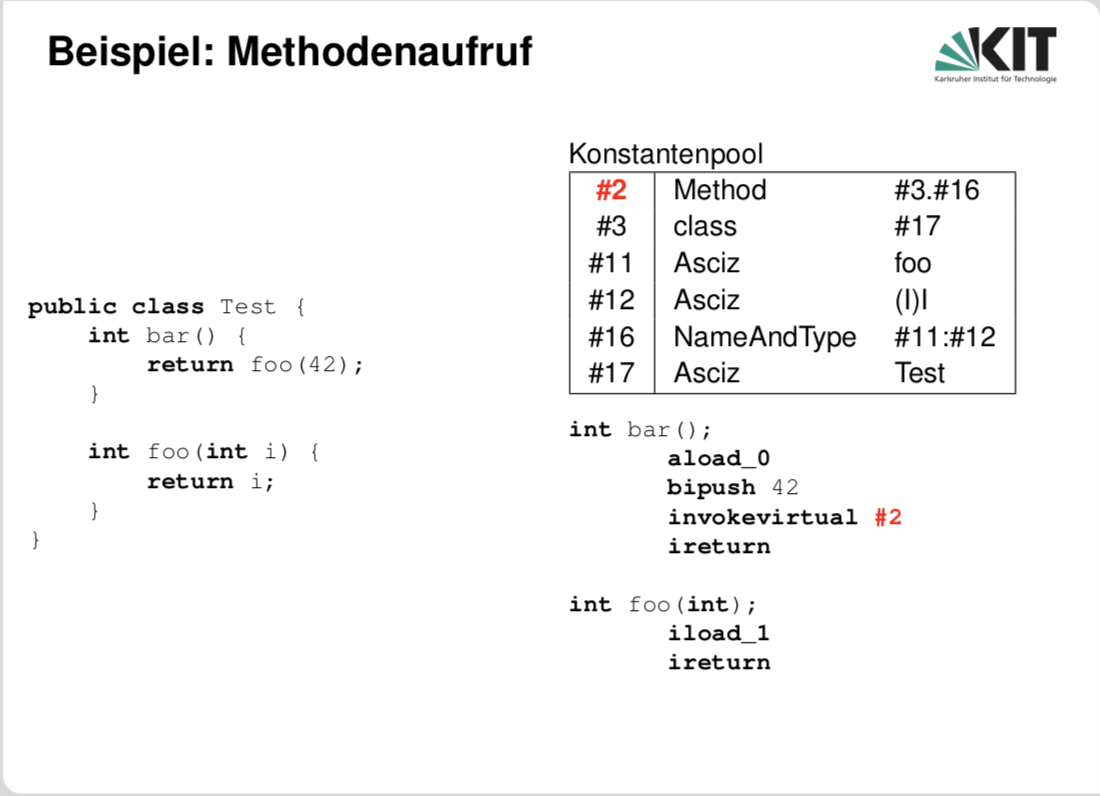
\includegraphics[width=\columnwidth]{images/byte_code_call.png}
\textbf{Conditional jumps:}
\begin{lstlisting}[language=JVMIS]
if_icmpeq target // Jump if equal
if_icmpne target // Jump if NOT equal
if_icmpge target // Jump if equal or greater than
if_icmpgt target // Jump greater than
if_icmple target // Jump if equal or less than
if_icmplt target // Jump if less than
\end{lstlisting}